\subsection{Language Model}
\begin{frame}{\insertsubsection}{Information retrieval goal}
    \begin{itemize}
        \item We want to find relevant documents based on words in a query
        \begin{equation*}\label{eq:query_prob}
	        P(q|d) = \prod_{w \in q} P(w|d)
        \end{equation*}
    \end{itemize}
\end{frame}

\begin{frame}{\insertsubsection}{Explanation}
    \only<1>{
    \begin{equation*}\label{eq:word_prob}
    	P(w|d) = \frac{N_d}{N_d + \lambda} \cdot \frac{tf(w,d)}{N_d} + (1 - \frac{N_d}{N_d + \lambda}) \cdot \frac{tf(w,D)}{N_D}
    \end{equation*}
    \begin{itemize}
        \item $d$ = document
        \item $N_d$ = Number of words in $d$
        \item $\lambda$ is the average document length 
        \item $D$ = Corpus
    \end{itemize}
    }
    \only<2>{
    \begin{equation*}\label{eq:word_prob}
    	P(w|d) = \underbrace{\frac{N_d}{N_d + \lambda}}_{\text{weight term}} \cdot \frac{tf(w,d)}{N_d} + \underbrace{(1 - \frac{N_d}{N_d + \lambda})}_{\text{inverse weight term}} \cdot \frac{tf(w,D)}{N_D}
    \end{equation*}
    \begin{itemize}
        \item $d$ = document
        \item $N_d$ = Number of words in $d$
        \item $\lambda$ is the average document length 
        \item $D$ = Corpus
    \end{itemize}
    }
    \only<3>{
    \begin{equation*}\label{eq:word_prob}
    	P(w|d) = \underbrace{\frac{N_d}{N_d + \lambda}}_{\text{weight term}} \cdot \underbrace{\frac{tf(w,d)}{N_d}}_{\text{\% of w in d}} + \underbrace{(1 - \frac{N_d}{N_d + \lambda})}_{\text{inverse weight term}} \cdot \underbrace{\frac{tf(w,D)}{N_D}}_{\text{\% w in D}}
    \end{equation*}
    \begin{itemize}
        \item $d$ = document
        \item $N_d$ = Number of words in $d$
        \item $\lambda$ is the average document length 
        \item $D$ = Corpus
    \end{itemize}
    }
    \only<4>{
    \begin{equation*}\label{eq:word_prob}
    	P(w|d) = \underbrace{\frac{N_d}{N_d + \lambda}}_{\text{weight term}} \cdot \underbrace{\frac{tf(w,d)}{N_d}}_{\text{\% of w in d}} + \underbrace{(1 - \frac{N_d}{N_d + \lambda})}_{\text{inverse weight term}} \cdot \underbrace{\frac{tf(w,D)}{N_D}}_{\text{\% w in D}}
    \end{equation*}
    \begin{itemize}
        \item $d$ = document
        \item $N_d$ = Number of words in $d$
        \item $\lambda$ is the average document length 
        \item $D$ = Corpus
    \end{itemize}
    }
    \only<5>{
        \begin{itemize}
            \item Favors high percentage of a word in a document or corpus
        \end{itemize}
    }
\end{frame}

\subsection{TF-IDF}
\begin{frame}{\insertsubsection}{Explanation}
    \only<1>{
    \begin{equation*}\label{eq:tfidf}
    	\text{tf-idf}(t, d, D) = \text{tf}(t, d) \cdot \text{idf}(t, D)
    \end{equation*}
    \begin{itemize}
        \item $t$ = Term
        \item $d$ = Document
        \item $D$ = Corpus
    \end{itemize}
    }
    \only<2>{
    \begin{equation*}\label{eq:tfidf}
    	\text{tf-idf}(t, d, D) = \text{tf}(t, d) \cdot log \frac{|\{d \in D\}|}{|\{d \in D : t \in d\}|}
    \end{equation*}
    }
\end{frame}

\begin{frame}{\insertsubsection}{Summary}
    \begin{itemize}
        \item Favors high usage of unique word(s) in a document or corpus
    \end{itemize}
\end{frame}


\subsection{BM25}
\begin{frame}{\insertsubsection}{Explanation}
    \only<1>{
    \begin{equation*}\label{eq:bm25}
    	\text{bm25}(d, q) = \sum_{i=1}^{n}\text{idf}(q_i) \cdot \frac{\text{tf}(q_i, d) \cdot (k_1 + 1)}{\text{tf}(q_i, d) + k_1 \cdot (1 - b + b \cdot \frac{|d|}{avgdl})}
    \end{equation*}
    \begin{itemize}
        \item $b$ adjust the sensitivity of varying document lengths
        \item $k_1$ adjust how quickly a term is saturated 
    \end{itemize}
    }
    
    \only<2>{
    \begin{equation*}\label{eq:bm25}
    	\text{bm25}(d, q) = \sum_{i=1}^{n}\text{idf}(q_i) \cdot \frac{\text{tf}(q_i, d) \cdot (1.5 + 1)}{\text{tf}(q_i, d) + 1.5 \cdot (1 - 0.75 + 0.75 \cdot \frac{|d|}{avgdl})}
    \end{equation*}
    }
\end{frame}

\begin{frame}{\insertsubsection}{Summary}
    \begin{itemize}
        \item Similar to tf-idf but with some other focus points
        \begin{itemize}
            \item Document length 
            \item Word saturation 
        \end{itemize}
    \end{itemize}
\end{frame}



\subsection{Combination of methods}
\begin{frame}{\insertsubsection}{How to combine?}
    \begin{figure}
    \centering
    \begin{tikzpicture}
        \matrix [matrix of nodes,row sep=0mm, set common column={2,3,4,5,7}{nodes={rectangle,draw,minimum width=3em}}, set common row={1,3} {nodes={draw=none}}, ] (O)
        {
            & $D_0$ & $D_1$ & $D_2$ & $D_3$ &  \\
            BM25 (b) & $S^{b}_{D_0}$ & $S^{b}_{D_1}$ & $S^{b}_{D_2}$ & $S^{b}_{D_3}$ & \dots \\
            & + & + & + & + & \\
            PR (p) & $S^{p}_{D_0}$ & $S^{p}_{D_1}$ & $S^{p}_{D_2}$ & $S^{p}_{D_3}$ & \dots \\[8mm]
            BM25+PR & $S^{b}_{D_0} + S^{p}_{D_0} $ & $S^{b}_{D_1} + S^{p}_{D_1} $ & $S^{b}_{D_2} + S^{p}_{D_2} $ & $S^{b}_{D_3} + S^{p}_{D_3} $ &  \dots \\
        };
        \foreach\x in{2,3,4,5}{\draw[my arrow] (O-4-\x) to (O-5-\x);}
    \end{tikzpicture}
\end{figure}
    \vspace{0.5cm}
    \only<2>{
        \begin{itemize}
            \item $ t \cdot A + (1-t) \cdot B $
        \end{itemize}
    }
\end{frame}

\section{Query Generation}
\begin{frame}{\insertsection}{Types of queries}
    \begin{itemize}
        \item Document query
        \begin{itemize}
            \item Specificity - Finding a specific document
        \end{itemize}
        \item Topic query
        \begin{itemize}
            \item Generality - Finding topic relevant documents
        \end{itemize}
    \end{itemize}
\end{frame}

\subsection{Document Query}
\begin{frame}{\insertsubsection}{Generation}
    \tikzstyle{document} = [circle, rounded corners ,text centered, draw=black]
\tikzstyle{corpus} = [draw,thick,minimum width=1cm,minimum height=4cm]
\tikzstyle{tf-idf} = [draw,thick,minimum width=1cm,minimum height=1cm]

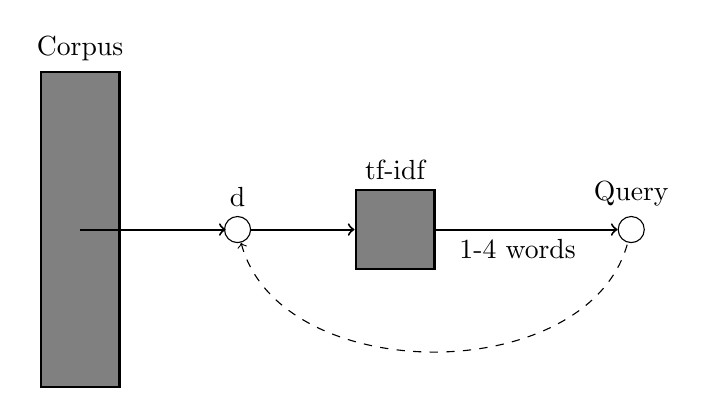
\begin{tikzpicture}
    \node [fill=gray, label={Corpus}] (corpus) at (0,0) [corpus] {};
    \onslide<2->{
        \node [document, label={d}] (doc) at (2, 0) {};
        \draw [line width=0.25mm, ->] (0,0) -> (1.85,0) node [right] {};
    };
    \onslide<3->{
        \node [fill=gray, label={tf-idf}] (tf-idf) at (4,0) [tf-idf] {};
        \draw [line width=0.25mm, ->] (doc) -> (tf-idf)  {};
    };
    \onslide<4->{
        \node [document, label={Query}] (Query) at  (7, 0) {};
        \draw [line width=0.25mm, ->] (tf-idf) -- node[below] {$1$-$4$ words} ++(2.6,0) -- (Query);
    };
    \onslide<5->{
        \path (doc) edge[bend right=75, dashed, <-] node [left] {} (Query);
    }
\end{tikzpicture}
\end{frame}

\subsection{Topic Query}
\begin{frame}{\insertsubsection}{Generation}
    \tikzstyle{document} = [circle, rounded corners ,text centered, draw=black]
\tikzstyle{topic} = [draw,thick,minimum width=1cm,minimum height=4cm]
\tikzstyle{tf-idf} = [draw,thick,minimum width=1cm,minimum height=1cm]

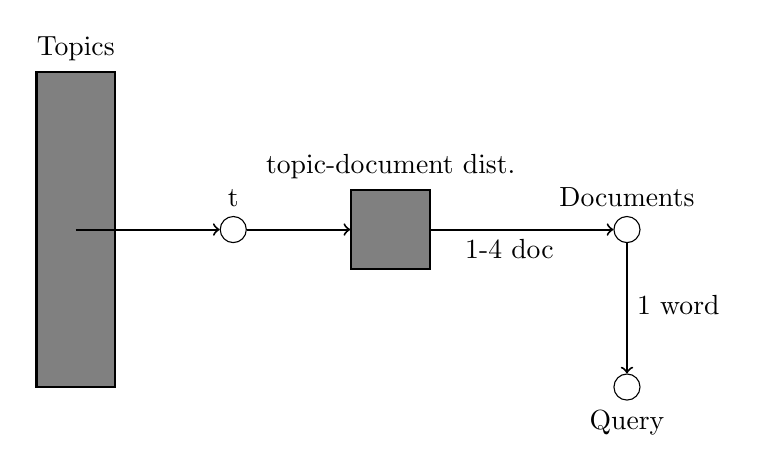
\begin{tikzpicture}
    \node [fill=gray, label={Topics}] (topic) at (0,0) [topic] {};
    \onslide<2->{
        \node [document, label={t}] (top) at (2, 0) {};
        \draw [line width=0.25mm, ->] (0,0) -> (top) node [right] {};
    };
    \onslide<3->{
        \node [fill=gray, label={topic-document dist.}] (dist) at (4,0) [tf-idf] {};
        \draw [line width=0.25mm, ->] (top) -> (dist)  {};
    };
    \onslide<4->{
        \node [document, label={Documents}] (documents) at  (7, 0) {};
        \draw [line width=0.25mm, ->] (dist) -- node[below] {1-4 doc} ++(2.5,0) -- (documents);
    };
    \onslide<5->{
        \node [document, label=below:Query] (query) at  (7, -2) {};
        \draw [line width=0.25mm, ->] (documents) -- node[right] {1 word} ++(0,-1.75) -- (query);
    };
\end{tikzpicture}
    \only<6>{
        \begin{itemize}
            \item Sample the topic-word distribution instead
        \end{itemize}
    }
\end{frame}